\documentclass[letterpaper,10pt,serif, draftclsnofoot,onecolumn, compsoc, titlepage]{IEEEtran}

\usepackage{graphicx}
\usepackage{amssymb}
\usepackage{amsmath}
\usepackage{amsthm}

\usepackage{alltt}
\usepackage{float}
\usepackage{color}
\usepackage{url}

\usepackage{balance}
\usepackage[TABBOTCAP, tight]{subfigure}
\usepackage{enumitem}
\usepackage{pstricks, pst-node}

\usepackage{geometry}
\geometry{margin=.75in}

\usepackage{hyperref}
\usepackage{vertabim}

% This method for displaying a relational schema was found on Stack Exchange from user Bruno Vandekerkhove
% tex.stackexchange.com/questions/296948/creating-a-relational-database-schema
\usepackage{tikz}
\usetikzlibrary{shapes, positioning, calc}
\colorlet{lightgray}{gray!20}

\usepackage{caption}
\usepackage{listings}

\begin{document}

% Adding these from the template in Annex C of the standard
% Some may not apply, but I'm sure most will
\section{Kyle- Database Management}
\subsection{Database organization}
The database will be organized around the core elements of surveys, questions, and responders.
These will compromise the three core tables in the database, with other tables functioning as relationships or specializations of these core tables.
All tables contain unique IDs as their primary key, and each ID is a non-negative integer.

The Survey table will contain the survey\_id as its primary key to identify each individual Survey.
Each Survey will also contain a string attribute for the title.

The Question table represents any individual kind of question.
It's attributes include a unique question\_id to serve as its primary key and the question's text as a string attribute.
The question text will be generated through the survey generation process and be stored here when the Question is created.

Surveys and Questions have a many-to-many relationship: Questions can exist in many different Surveys and Surveys contain many different questions.
To create this relationship in our database, a Contains table will exist.
The Contains table's primary key will be a combination of a survey\_id and a question\_id to correspond a questions use in a survey.
The question\_id and survey\_id individually can be used in other Contains entries, but since surveys don't have the same question multiple times, the combination will be unique for each table entry.

The Responder table will store information on the individual responders.
This includes a unique responder\_id for the primary key, two string attributes for first\_name and last\_name, the birthdate as a date attribute, and a non-negative integer attribute for the age derived from the birthdate and the current date.
The age can be updated or refreshed when necessary.
The Responder table has two specializations: a Student and a Parent.
A Parent does not contain any extra information, but a Student contains a parent1\_id and a parent2\_id to correspond to both of its parents.
The specialization is to allow for more accurate and specified queries of students and parents separately or together.
As specializations, they also contain a matching responder\_id to their corresponding Responder table entry.

To save responses, a Response table will exist.
This functions as the many-to-many relationship between Responders and Questions, but also stores the answer provided for the question.
The Response table has three specializations for each of the possible types of questions: Multiple\_Choice, Matrix, and Text.
Multiple\_Choice entries contain a character attribute for the answer, Matrix entries use a non-negative integer attribute, and Text entries use a string attribute.
Each of these specializations also contain the response\_id for the corresponding entry.

The below diagram outlines the relational database schema described above.

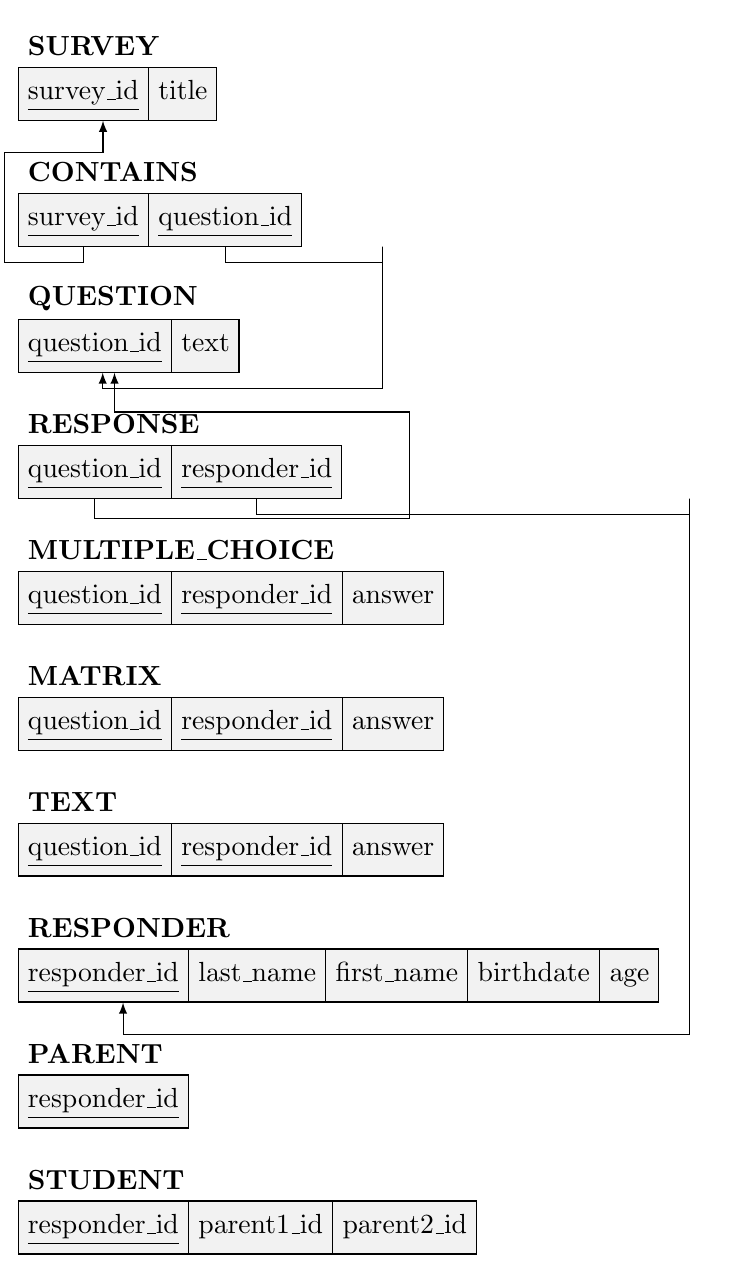
\begin{tikzpicture}[relation/.style={rectangle split, rectangle split parts=#1, rectangle split part align=base, draw, anchor=center, align=center, text height=3mm, text centered}]\hspace*{-0.3cm}

% Relations

\node (surveytitle) {\textbf{SURVEY}};
\node [relation=2, rectangle split horizontal, rectangle split part fill={lightgray!50}, anchor=north west, below=0.6cm of surveytitle.west, anchor=west] (survey)
{\underline{survey\_id}%
\nodepart{two}		title};

\node [below=1cm of survey.west, anchor=west] (containstitle) {\textbf{CONTAINS}};
\node [relation=2, rectangle split horizontal, rectangle split part fill={lightgray!50}, anchor=north west, below=0.6cm of containstitle.west, anchor=west] (contains)
{\underline{survey\_id}
\nodepart{two}	\underline{question\_id}};

\node [below=1cm of contains.west, anchor=west] (questiontitle) {\textbf{QUESTION}};
\node [relation=2, rectangle split horizontal, rectangle split part fill={lightgray!50}, anchor=north west, below=0.6cm of questiontitle.west, anchor=west] (question)
{\underline{question\_id}%
\nodepart{two}		text};

\node [below=1cm of question.west, anchor=west] (responsetitle) {\textbf{RESPONSE}};
\node [relation=2, rectangle split horizontal, rectangle split part fill={lightgray!50}, anchor=north west, below=0.6cm of responsetitle.west, anchor=west] (response)
{\underline{question\_id}%
\nodepart{two}		\underline{responder\_id}};

\node [below=1cm of response.west, anchor=west] (multiplechoicetitle) {\textbf{MULTIPLE\_CHOICE}};
\node [relation=3, rectangle split horizontal, rectangle split part fill={lightgray!50}, anchor=north west, below=0.6cm of multiplechoicetitle.west, anchor=west] (multiplechoice)
{\underline{question\_id}%
\nodepart{two}		\underline{responder\_id}
\nodepart{three}	answer};

\node [below=1cm of multiplechoice.west, anchor=west] (matrixtitle) {\textbf{MATRIX}};
\node [relation=3, rectangle split horizontal, rectangle split part fill={lightgray!50}, anchor=north west, below=0.6cm of matrixtitle.west, anchor=west] (matrix)
{\underline{question\_id}%
\nodepart{two}		\underline{responder\_id}
\nodepart{three}	answer};

\node [below=1cm of matrix.west, anchor=west] (texttitle) {\textbf{TEXT}};
\node [relation=3, rectangle split horizontal, rectangle split part fill={lightgray!50}, anchor=north west, below=0.6cm of texttitle.west, anchor=west] (text)
{\underline{question\_id}%
\nodepart{two}		\underline{responder\_id}
\nodepart{three}	answer};

\node [below=1cm of text.west, anchor=west] (respondertitle) {\textbf{RESPONDER}};
\node [relation=5, rectangle split horizontal, rectangle split part fill={lightgray!50}, anchor=north west, below=0.6cm of respondertitle.west, anchor=west] (responder)
{\underline{responder\_id}%
\nodepart{two}		last\_name
\nodepart{three}	first\_name
\nodepart{four}	birthdate
\nodepart{five}		age};

\node [below=1cm of responder.west, anchor=west] (parenttitle) {\textbf{PARENT}};
\node [relation=1, rectangle split horizontal, rectangle split part fill={lightgray!50}, anchor=north west, below=0.6cm of parenttitle.west, anchor=west] (parent)
{\underline{responder\_id}};

\node [below=1cm of parent.west, anchor=west] (studenttitle) {\textbf{STUDENT}};
\node [relation=3, rectangle split horizontal, rectangle split part fill={lightgray!50}, anchor=north west, below=0.6cm of studenttitle.west, anchor=west] (student)
{\underline{responder\_id}%
\nodepart{two}		parent1\_id
\nodepart{three}	parent2\_id};

% Foreign keys

\draw[-latex] (contains.one south) -- ++(0,-0.2) -| ($(contains.one south) + (-1,0)$) |- ($(survey.one south) + (0.25,-0.40)$) -| ($(survey.one south) + (0.25,0)$);

\draw[-latex] (contains.two south) -- ++(0,-0.2) -| ($(contains.two south) + (2,0)$) |- ($(question.one south) + (0.25,-0.20)$) -| ($(question.one south) + (0.10,0)$);

\draw[-latex] (response.one south) -- ++(0,-0.25) -| ($(response.one south) + (4,0)$) |- ($(question.one south) + (0.25,-0.50)$) -| ($(question.one south) + (0.25,0)$);

\draw[-latex] (response.two south) -- ++(0,-0.2) -| ($(response.two south) + (5.50,0)$) |- ($(responder.one south) + (0.25,-0.40)$) -| ($(responder.one south) + (0.25,0)$);

\end{tikzpicture}
\captionof{figure}{The relational database schema}

\subsection{Database creation}
Each table will be created with the following SQL syntax.
In particular, tables will use AUTO INCREMENT to automatically increment and create IDs.
They will also be done in the following order because some tables reference others.
\lstset{language=SQL,breaklines=true}
\begin{lstlisting}
CREATE TABLE Survey
(
 survey_id int NOT NULL AUTO_INCREMENT
 title varchar(255)
 PRIMARY KEY (survey_id)
)

CREATE TABLE Question
(
 question_id int NOT NULL AUTO_INCREMENT
 text varchar(1020) NOT NULL
 PRIMARY KEY (question_id)
)

CREATE TABLE Contains
(
 survey_id int NOT NULL
 question_id int NOT NULL
 PRIMARY KEY (survey_id, question_id)
 FOREIGN KEY (survey_id) REFERENCES Survey(survey_id)
 FOREIGN KEY (question_id) REFERENCES Question(question_id)
)

CREATE TABLE Responder
(
 responder_id int NOT NULL AUTO_INCREMENT
 first_name varchar(255) NOT NULL
 last_name varchar(255) NOT NULL
 birthdate date
 age int
 PRIMARY KEY (responder_id)
)

CREATE TABLE Parent
(
 responder_id int NOT NULL
 PRIMARY KEY (responder_id)
 FOREIGN KEY (responder_id) REFERENCES Responder(responder_id)
)

CREATE TABLE Student
(
 responder_id int NOT NULL
 parent1_id int
 parent2_id int
 PRIMARY KEY (responder_id)
 FOREIGN KEY (responder_id) REFERENCES Responder(responder_id)
 FOREIGN KEY (parent1_id) REFERENCES Parent(responder_id)
 FOREIGN KEY (parent2_id) REFERENCES Parent(responder_id)
)

CREATE TABLE Response
(
 question_id int NOT NULL
 responder_id int NOT NULL
 PRIMARY KEY (question_id, responder_id)
 FOREIGN KEY (question_id) REFERENCES Question(question_id)
 FOREIGN KEY (responder_id) REFERENCES Responder(responder_id)
)
\end{lstlisting}


%CREATE TABLE Multiple_Choice
%(
 % question_id int NOT NULL
  %responder_id int NOT NULL
% answer char(1)
 %PRIMARY KEY (question_id, responder_id)
 %FOREIGN KEY (question_id) REFERENCES Question(question_id)
 %FOREIGN KEY (responder_id) REFERENCES Responder(responder_id)
%)

%CREATE TABLE Matrix
%(
 %question_id int NOT NULL
 %responder_id int NOT NULL
 %answer int
% PRIMARY KEY (question_id, responder_id)
 %FOREIGN KEY (question_id) REFERENCES Question(question_id)
 %FOREIGN KEY (responder_id) REFERENCES Responder(responder_id)
%)

%CREATE TABLE Text
%(
 %question_id int NOT NULL
 %responder_id int NOT NULL
 %answer varchar(1020)
 %PRIMARY KEY (question_id, responder_id)
 %FOREIGN KEY (question_id) REFERENCES Question(question_id)
 %FOREIGN KEY (responder_id) REFERENCES Responder(responder_id)
%)

\subsection{Database interaction}
To allow for interaction between the survey and report generation, an API will need to be created to work with both.
The API will be written in PHP since PHP provides functionality to generate SQL queries with a database using \texttt{mysqli} objects and the \texttt{query()} function.
\subsubsection{Interacting with the survey generation}
Since the survey generation will be done using JSON, the API will need to get the POST information as the JSON object and parse it for a SQL INSERT.
It will do so using the following design:
\begin{enumerate}
	\item Generate a string \texttt{sql\_query} for the SQL query setting up the INSERT query with `INSERT INTO ` and adding the name of the table from the POST information.
	\item Because each table has different sets of attributes, a switch statement will be used to check the table name and add the necessary string to \texttt{sql\_query} (this switch statement will take the value from the POST and convert it all to lowercase).
	\begin{enumerate}
		\item The Survey table will add `(title)`.
		\item The Contains table will add `(survey\_id, question\_id)`.
		\item The Question table will add `(text)`.
		\item The Response table will add `(question\_id, responder\_id)`.
		\item The Multiple\_Choice, Matrix, and Text tables will add `(question\_id, responder\_id, answer)`.
		\item The Responder table will add `(last\_name, first\_name, birthdate, age)`
		\item The Student table will add `(responder\_id, parent1\_id, parent2\_id)`.
		\item The Parent table will add `(responder\_id)`.
	\end{enumerate}
	\item The string `VALUES ` will be appended to \texttt{sql\_query}.
	\item A while loop will wrap around the following process to account for multiple entries being added to the table.
	\begin{enumerate}
		\item There will be another switch structure to determine the number of values that will be inserted based on the table to be inserted into:
		\begin{enumerate}
			\item The Survey, Question, and Parent tables will read one value and add `(\emph{value1}),` to \texttt{sql\_query} accordingly.
			\item The Contains and Reponse tables will read two values and add `(\emph{value1}, \emph{value2}),` to \texttt{sql\_query}.
			\item The Multiple\_Choice, Matrix, Text, and Student tables will read three values and add `(\emph{value1}, \emph{value2}, \emph{value3}),` to \texttt{sql\_query}.
			\item The Responder table will read four values and add `(\emph{value1}, \emph{value2}, \emph{value3}, \emph{value4}, \emph{value5}),` to \texttt{sql\_query}.
		\end{enumerate}
	\end{enumerate}
	\item After the loop, the last character of \texttt{sql\_query} should be a comma, and it will be replaced with a semicolon.
	\item After the string has been completed, a mysqli object \texttt{conn} will be created that connects to the server the database is stored on.
	\item A call to \texttt{conn}'s function \texttt{query()}, passing \texttt{sql\_query} as the argument query string.
				The result will be stored in a variable called \texttt{result}.
	\item There will be a check on if the value of \texttt{result} is true.
	\begin{enumerate}
		\item If it is true, then display a success message.
		\item If it is not true, then display an error message.
	\end{enumerate}
	\item Lastly, \texttt{connection} will be closed.
\end{enumerate}

\subsubsection{Interacting with report generation}
% *** WORK IN PROGRESS ***
\begin{enumerate}
	\item The API will receive the SQL query as a string and store it as \texttt{sql\_query}.
	\item A mysqli object \texttt{conn} will be created that connects to the server the database is stored on.
	\item A call to \texttt{conn}'s function \texttt{query()}, passing \texttt{sql\_query} as the argument query string.
				The result will be stored in a variable called \texttt{result}.
	\item There will be a check on if the value of \texttt{result} is true.
	\begin{enumerate}
		\item If it is true, then display a success message.
		\item If it is not true, then display an error message.
	\end{enumerate}
	\item \texttt{connection} will be closed.
	\item Lastly, \texttt{result} will be echoed.
\end{enumerate}

\end{document}